The most relevant parts of the source code and the resulting plots are written here, but the rest, and the code for plotting can be found in the attached Jupyter Notebook named "CLFA5.ipynb":
\begin{verbatim}
# This function has been taken from the lecture slides
def prior(x, prior_alpha, prior_beta):
    return beta.pdf(x, prior_alpha, prior_beta)

# This function has been taken from the lecture slides
def posterior(x, prior_alpha, prior_beta, sample):
    N = len(sample)
    y_N = sum(sample)
    delta = y_N + prior_alpha
    gamma = N - y_N + prior_beta
    return beta.pdf(x, delta, gamma)

# This function has been taken from the lecture slides
def draw_sample(r, num):
    return np.random.binomial(1,r,num)

# Parts of this code has been taken from
# lecture slides and adapted for my use
def plotPrior(alpha, pbeta, accuracy):
    xsamples = np.linspace(0,1,accuracy+1)
    PriorVals = prior(xsamples, alpha, pbeta)
    
    plt.plot(xsamples, PriorVals, color = 'orange', label="Prior")
    plt.legend()
    return PriorVals

# Parts of this code has been taken from
# lecture slides and adapted for my use
def plotPosterior(alpha, pbeta, r, iterations, sample, frequency):
    xsamples = np.linspace(0,1,1000)
    PosteriorVals = np.zeros([iterations, len(xsamples)])
    PlottedSampleSizes = np.arange(1,iterations+1,1)
    colors = colors = cm.cool(np.linspace(0,1,np.max(PlottedSampleSizes)+1))
    
    for i in range(iterations):
        PosteriorVals[i,:] = posterior(xsamples, alpha, pbeta, sample[:i+1])

    for i in PlottedSampleSizes:
        if (i%frequency == 0 or i <= 5):
            plt.plot(xsamples,PosteriorVals[i-1,:],color=colors[i],label=f'Posterior {i}')
   
    plt.xlabel('r')
    plt.ylabel('P(r | sample)')
    plt.title(f'Posterior with r = {r}, alpha = {alpha} and beta = {pbeta}')
    return PosteriorVals
\end{verbatim}
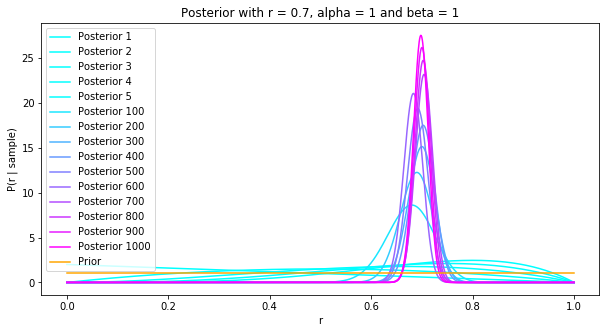
\includegraphics[width=\linewidth]{2a.png}
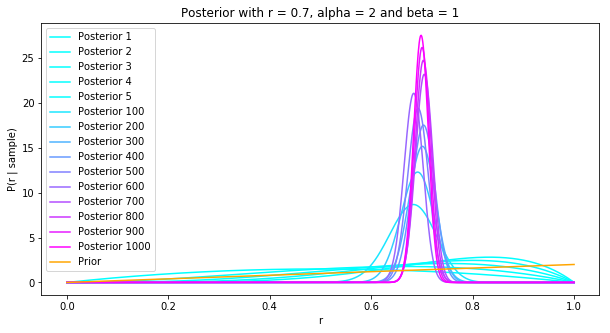
\includegraphics[width=\linewidth]{2b.png}
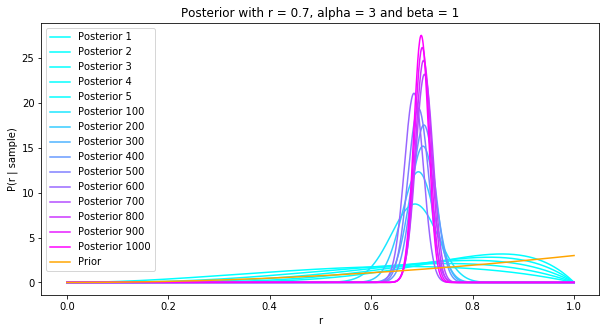
\includegraphics[width=\linewidth]{2c.png}